
\providecommand{\Hom}{\operatorname{Hom}}
\providecommand{\rvTranspose}[1]{\ulcorner #1\urcorner}%

\section{极限与余极限}\label{sec:f-limits-and-colimits}

本节中，我们扩展\cref{prop:limits-as-terminal-cones}，证明以\trSimplicialSet{}为索引、
取值于\trQuasiCategory{}的\trDiagram{}的\trLimit{}的综合定义，与 Joyal \cite[4.5]{bib61} 最先引入的
解析定义相一致。我们证明\trLimit{}锥的四个综合定义——(i) 最初的%
\cref{def:limit-colimit-cones}；(ii) 出现于\cref{prop:absolute-right-lifting-res}中的那个；(iii) 出现于\cref{def:limit-colimit-diagrams}与\cref{prop:limit-pointwise-extension-transpose}中的那个；以及 (iv) 来自%
\cref{prop:limits-as-terminal-cones}的那个——与一个解析定义 (v)（即 Joyal
的定义）之间的等价性。此时，凭借刚才所引的诸结果以及%
\cref{prop:terminal-element-equivalences}，除了陈述该结果并为其各组成部分
提供出处之外，已无事可做。

\begin{proposition}\label{prop:limit-cone-equivalences}
考虑\trQuasiCategory{}之间的\trFunctor{} $d\colon J\to A$ 以及\trCone{} $\lambda\colon\Delta\ell\Rightarrow d$。
以下条件等价：
\begin{enumerate}[label=(\roman*)]
\item 对 $(\ell,\lambda)$ 定义一个\trAbsoluteRightLifting{}图表
\begin{center}
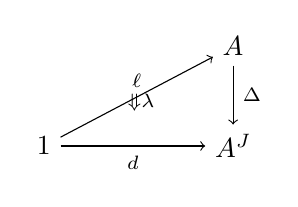
\begin{tikzpicture}[x=1.9em,y=1.5em]
  \node (a)  at (3.6,1.2)  {$A$};
  \node (aj) at (3.6,-1.2) {$A^{J}$};
  \node (o)  at (0,-1.2)   {$1$};
  \draw[->] (o) -- node[above]{$\scriptstyle\ell$} (a);
  \draw[->] (a) -- node[right]{$\scriptstyle\Delta$} (aj);
  \draw[->] (o) -- node[below]{$\scriptstyle d$} (aj);
  \node at (1.85,-0.15) {$\scriptstyle\Downarrow\lambda$};
\end{tikzpicture}
\end{center}
\item \trCone{} $\rvTranspose{\lambda}\colon 1\to A^{J\triangleleft}$ 定义一个%
\trAbsoluteRightLifting{}图表
\begin{center}
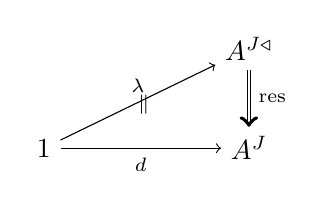
\begin{tikzpicture}[x=1.9em,y=1.5em]
  \node (ajl) at (3.9,1.2)  {$A^{J\triangleleft}$};
  \node (aj)  at (3.9,-1.2) {$A^{J}$};
  \node (o)   at (0,-1.2)   {$1$};
  \draw[->] (o) -- node[above]{$\scriptstyle\rvTranspose{\lambda}$} (ajl);
  \draw[double,->] (ajl) -- node[right]{$\scriptstyle\mathrm{res}$} (aj);
  \draw[->] (o) -- node[below]{$\scriptstyle d$} (aj);
  \node at (1.9,-0.15) {$\scriptstyle\parallel$};
\end{tikzpicture}
\end{center}
\item \trCone{} $\lambda\colon\ell!\Rightarrow d$ 定义一个逐点右扩张图表
\begin{center}
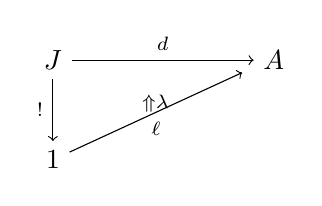
\begin{tikzpicture}[x=1.9em,y=1.5em]
  \node (j) at (0,1.2)   {$J$};
  \node (a) at (4.2,1.2) {$A$};
  \node (o) at (0,-1.2)  {$1$};
  \draw[->] (j) -- node[above]{$\scriptstyle d$} (a);
  \draw[->] (j) -- node[left]{$\scriptstyle !$} (o);
  \draw[->] (o) -- node[below,pos=0.5]{$\scriptstyle\ell$} (3.6,0.9);
  \node at (1.95,0.15) {$\scriptstyle\Uparrow\lambda$};
\end{tikzpicture}
\end{center}
\item \begingroup
\emergencystretch=3em
\trCone{}的\trQuasiCategory{} $\Hom_{A^{J}}(\Delta,d)$ 容有一个\trTerminal{}\trElement
$\rvTranspose{\lambda}\colon 1\to\Hom_{A^{J}}(\Delta,d)$，表示\trCone
$\lambda\colon\Delta\ell\Rightarrow d$。
\par\endgroup
\item \trQuasiCategory{} $A_{/d}$ 容有一个\trTerminal{}\trElement{} $\rvTranspose{\lambda}\colon 1\to A_{/d}$，
经转置定义 $d$ 到\trDiagram{} $J^{\triangleleft}\to A$ 的一个\trExtension
\begin{center}
\begin{tikzpicture}[x=1.9em,y=1.5em]
  \node (j)  at (2.2,1.4)  {$J$};
  \node (jl) at (0,-1.0)   {$J^{\triangleleft}$};
  \node (a)  at (4.6,-1.0) {$A$};
  \draw[right hook->] (j) -- (jl);
  \draw[->] (j) -- node[right,pos=0.6]{$\scriptstyle d$} (a);
  \draw[->] (jl) -- node[below]{$\scriptstyle\rvTranspose{\lambda}$} (a);
\end{tikzpicture}
\end{center}
\end{enumerate}
\end{proposition}

当这些条件成立时，以 $(\ell,\lambda)$ 或 $\rvTranspose{\lambda}$ 各种方式标记的
数据，定义了 $d$ 上的\textbf{\trLimit{}锥}。

注意，任何以\trSimplicialSet{}为索引、取值于\trQuasiCategory{}的\trDiagram{} $d'\colon J'\to A$，都可以沿一个
内\trAnodyneExtension，扩充为\trQuasiCategory{}之间的一个\trWeakEquivalence{}\trDiagram{} $d\colon J\to A$。或者在
(i)、(ii)、(iv)、(v) 诸情形中直接处理原始\trDiagram{}亦无任何代价，因为\trDiagram{}的\trQuasiCategory
$A^{J}\simeq A^{J'}$、\trCone{}的\trQuasiCategory{} $\Hom_{A^{J}}(\Delta,d)\simeq\Hom_{A^{J'}}(\Delta,d')$ 以及 $A_{/d}\simeq A_{/d'}$ 都是等价的。

\begin{proof}
(i) 与 (ii) 的等价性由\cref{prop:absolute-right-lifting-res}对任何%
\trInfinityCategory{} $A$ 与\trSimplicialSet{} $J$ 证明；而%
\trSimplicialSet{} $J^{\triangleleft}\coloneqq 1\star J$ 是\cref{def:join}中的\trJoin。(i) 与 (iii)
的等价性由\cref{prop:limit-pointwise-extension-transpose}对任何%
\trCartesianClosed{}\trInfinityCosmos{}证明。\cref{prop:limits-as-terminal-cones}证明了：对取值于任何%
\trInfinityCategory{}的任何\trDiagram{}，(i) 与 (iv) 之间的等价性都成立。

最后，(iv) 与 (v) 之间的等价性是\cref{prop:slices-cones-equivalence}所给出的、
卧于 $A$ 之上的\trQuasiCategory\trEquivalence{}
$\Hom_{A^{J}}(\Delta,d)\simeq A_{/d}$ 的一个推论；该命题给出 $d$ 之上\trCone{}的%
\trQuasiCategory{}的两个模型。最后一个要素是%
\cref{lem:equivalence-invariance-initial-elements}，它证明：这些%
\trQuasiCategory{}中若有一个容有\trTerminal{}\trElement{}，则两者皆然，因为%
\trTerminal{}\trElement{}被诸\trEquivalence{}保持。
\end{proof}

\subsection*{练习}

\begin{exercise}\label{ex:colimit-equivalences}
陈述并证明取值于\trQuasiCategory{}的\trDiagram{}的\trColimit{}的各种综合定义与解析定义之间的\trEquivalence。
\end{exercise}

